\documentclass[11pt,a4paper]{report}

% ============================================================
% PACKAGES
% ============================================================
\usepackage[T1]{fontenc}
\usepackage[utf8]{inputenc}
\usepackage[french]{babel}
\usepackage{lmodern}
\usepackage{geometry}
\geometry{left=2.5cm,right=2.5cm,top=2.5cm,bottom=2.5cm}

\usepackage{amsmath,amssymb,amsfonts,mathtools}
\usepackage{amsthm}
\usepackage{graphicx}
\usepackage{float}
\usepackage{xcolor}
\usepackage{tikz}
\usetikzlibrary{arrows.meta,positioning,calc}
\usepackage{hyperref}
\usepackage{enumitem}
\usepackage{listings}
\usepackage{caption}
\usepackage{subcaption}
\usepackage{booktabs}
\usepackage{array}
\usepackage{titlesec}
\usepackage{fancyhdr}
\usepackage[most]{tcolorbox}

% ============================================================
% HYPERREF
% ============================================================
\hypersetup{
  colorlinks=true,
  linkcolor=black,
  urlcolor=blue,
  citecolor=black
}

% ============================================================
% GLOBAL STYLE
% ============================================================
\setlength{\parindent}{0pt}
\setlength{\parskip}{0.45em}
\renewcommand{\baselinestretch}{1.08}
\hyphenpenalty=10000
\exhyphenpenalty=10000
\sloppy

% ============================================================
% COLORS
% ============================================================
\definecolor{bleufonce}{RGB}{28,39,55}
\definecolor{bleuclair}{RGB}{232,240,255}
\definecolor{or}{RGB}{176,132,45}
\definecolor{vertclair}{RGB}{230,247,238}
\definecolor{rougeclair}{RGB}{255,239,239}
\definecolor{grisclair}{RGB}{247,247,247}
\definecolor{codeblue}{RGB}{20,20,140}
\definecolor{codegray}{RGB}{120,120,120}
\definecolor{codepurple}{RGB}{120,0,160}
\definecolor{backcolour}{RGB}{245,245,240}

% ============================================================
% HEADER / FOOTER
% ============================================================
\pagestyle{fancy}
\setlength{\headheight}{24pt}
\fancyhf{}
\fancyhead[L]{Percolation par arêtes}
\fancyhead[R]{Projet de simulation}
\fancyfoot[C]{\thepage}
\renewcommand{\headrulewidth}{0.4pt}
\renewcommand{\headrule}{\hbox to\headwidth{\color{or}\leaders\hrule height \headrulewidth\hfill}}

% ============================================================
% CHAPTER AND SECTION STYLE
% ============================================================
\titleformat{\chapter}[display]
  {\normalfont\huge\bfseries\color{bleufonce}\centering}
  {\Large\color{or}\chaptername\ \thechapter}
  {0.25cm}
  {}
  [\vspace{0.25cm}{\color{or}\titlerule[1pt]}]

\titlespacing*{\chapter}{0pt}{-0.4cm}{0.9cm}

\titleformat{\section}
  {\normalfont\Large\bfseries\color{bleufonce}}
  {\thesection}
  {0.8em}
  {}
  [\vspace{0.15cm}{\color{or}\titlerule[0.6pt]}]

\titleformat{\subsection}
  {\normalfont\large\bfseries\color{bleufonce}}
  {\thesubsection}
  {0.8em}
  {}

% ============================================================
% BOXED THEOREM ENVIRONMENTS
% ============================================================
\tcbuselibrary{theorems}

\newtcbtheorem[number within=chapter]{definitionbox}{Définition}
{
  enhanced,
  colback=bleuclair,
  colframe=bleufonce,
  fonttitle=\bfseries,
  coltitle=white,
  colbacktitle=bleufonce,
  boxed title style={arc=2mm},
  sharp corners,
  boxrule=0.8pt
}{def}

\newtcbtheorem[number within=chapter]{propositionbox}{Proposition}
{
  enhanced,
  colback=vertclair,
  colframe=green!45!black,
  fonttitle=\bfseries,
  coltitle=white,
  colbacktitle=green!35!black,
  boxed title style={arc=2mm},
  sharp corners,
  boxrule=0.8pt
}{prop}

\newtcbtheorem[number within=chapter]{theorembox}{Théorème}
{
  enhanced,
  colback=yellow!8,
  colframe=or,
  fonttitle=\bfseries,
  coltitle=white,
  colbacktitle=or,
  boxed title style={arc=2mm},
  sharp corners,
  boxrule=0.8pt
}{thm}

\newtcbtheorem[number within=chapter]{remarkbox}{Remarque}
{
  enhanced,
  colback=rougeclair,
  colframe=red!45!black,
  fonttitle=\bfseries,
  coltitle=white,
  colbacktitle=red!45!black,
  boxed title style={arc=2mm},
  sharp corners,
  boxrule=0.8pt
}{rem}

\newenvironment{proofbox}
{\begin{tcolorbox}[colback=grisclair,colframe=black!25,title=\textbf{Démonstration},fonttitle=\bfseries,sharp corners,boxrule=0.6pt]}
{\end{tcolorbox}}

% ============================================================
% PYTHON STYLE
% ============================================================
\lstdefinestyle{pythonstyle}{
  language=Python,
  backgroundcolor=\color{backcolour},
  basicstyle=\ttfamily\scriptsize,
  keywordstyle=\color{codeblue}\bfseries,
  stringstyle=\color{codepurple},
  commentstyle=\color{codegray}\itshape,
  numbers=left,
  numberstyle=\tiny\color{codegray},
  stepnumber=1,
  numbersep=6pt,
  frame=single,
  rulecolor=\color{black!25},
  breaklines=true,
  breakatwhitespace=false,
  columns=fullflexible,
  keepspaces=true,
  showstringspaces=false,
  tabsize=2,
  captionpos=b,
  xleftmargin=0.5cm,
  xrightmargin=0.2cm
}
\lstset{style=pythonstyle}


% Captions in French
\addto\captionsfrench{
  \renewcommand{\tablename}{Tableau}
  \renewcommand{\figurename}{Figure}
}

% ============================================================
% CUSTOM COMMANDS
% ============================================================
\newcommand{\N}{\mathbb{N}}
\newcommand{\Z}{\mathbb{Z}}
\newcommand{\Pbb}{\mathbb{P}}
\newcommand{\E}{\mathbb{E}}
\newcommand{\Var}{\mathrm{Var}}
\newcommand{\thetaHat}{\widehat{\theta}}

% ============================================================
% DOCUMENT
% ============================================================
\begin{document}

% ============================================================
% COVER PAGE
% ============================================================
\begin{titlepage}
\thispagestyle{empty}

\begin{tikzpicture}[remember picture, overlay]

    % Diagonal band at the top left
    \fill[bleufonce] 
        (current page.north west) --
        ([xshift=3.8cm]current page.north west) --
        ([xshift=-1.2cm,yshift=-5.2cm]current page.north west) --
        (current page.north west);

    \fill[or] 
        ([xshift=3.4cm]current page.north west) --
        ([xshift=4.0cm]current page.north west) --
        ([xshift=-0.8cm,yshift=-5.2cm]current page.north west) --
        ([xshift=-1.3cm,yshift=-5.2cm]current page.north west);

    % Diagonal band at the bottom right
    \fill[bleufonce]
        (current page.south east) --
        ([xshift=-4.2cm]current page.south east) --
        ([xshift=1.4cm,yshift=5.2cm]current page.south east) --
        (current page.south east);

    \fill[or]
        ([xshift=-3.8cm]current page.south east) --
        ([xshift=-4.4cm]current page.south east) --
        ([xshift=0.9cm,yshift=5.2cm]current page.south east) --
        ([xshift=1.5cm,yshift=5.2cm]current page.south east);

\end{tikzpicture}

\centering

\vspace*{0.8cm}

{\large Paris 1 Panthéon-Sorbonne University\par}
\vspace{0.15cm}
{\large U.F.R. 27 -- Mathematics and Computer Science\par}

\vspace{2.1cm}

{\large\scshape Rapport de projet\par}
\vspace{0.15cm}
{\large\scshape Probabilités, simulation et théorie des graphes\par}
\vspace{0.15cm}
{\large\scshape Projet académique\par}

\vspace{1.9cm}

{\Large\bfseries\color{or} THÈME\par}

\vspace{0.4cm}

{\Huge\bfseries\color{bleufonce}
Percolation par arêtes :\\[0.2cm]
Simulation, probabilité de croisement et dualité
\par}

\vfill

\vspace{-1.2cm}

\noindent
\begin{minipage}[t]{0.45\textwidth}
\raggedright
{\large Réalisé par :\par}
\vspace{0.35cm}
\begin{itemize}
    \item Marc SU
\end{itemize}
\end{minipage}
\hfill
\begin{minipage}[t]{0.45\textwidth}
\raggedright
{\large Axes du projet :\par}
\vspace{0.35cm}
\begin{itemize}
    \item Percolation par arêtes
    \item Simulation Monte Carlo
    \item Dualité planaire
\end{itemize}
\end{minipage}

\vspace{1.5cm}

{\large Année universitaire 2025 -- 2026\par}

\end{titlepage}

% ============================================================
% EXECUTIVE SUMMARY
% ============================================================
\chapter*{Résumé exécutif}
\addcontentsline{toc}{chapter}{Résumé exécutif}

Ce rapport présente une étude de la percolation par arêtes sur une grille finie. Chaque arête est déclarée ouverte indépendamment avec une probabilité $p$, et l'objectif principal consiste à déterminer s'il existe un chemin ouvert reliant le bord gauche au bord droit de la grille.

Le projet combine trois dimensions complémentaires :
\begin{itemize}
    \item une modélisation probabiliste fondée sur des variables aléatoires de Bernoulli indépendantes ;
    \item une simulation informatique utilisant une exploration de graphe par parcours en largeur ;
    \item une analyse théorique de la probabilité de croisement $\theta_n(p)$, incluant la croissance en fonction de $p$, des bornes probabilistes et un argument de dualité planaire.
\end{itemize}

La partie numérique estime la probabilité de croisement par simulation Monte Carlo pour plusieurs tailles de grilles. Les résultats mettent en évidence une transition rapide autour de $p=1/2$, ce qui est cohérent avec le seuil critique connu pour la percolation par arêtes sur le réseau carré.

\newpage

% ============================================================
% TABLE OF CONTENTS
% ============================================================
\tableofcontents
\newpage

% ============================================================
% CHAPTER 1
% ============================================================
\chapter{Description du modèle et simulation}

\section{Percolation par arêtes sur une grille finie}

On considère une grille carrée finie de taille $n$. L'ensemble des sommets est défini par
\[
V_n=\{0,1,\ldots,n\}\times\{0,1,\ldots,n\}.
\]
Deux sommets sont reliés par une arête lorsque leur distance euclidienne est égale à $1$. L'ensemble des arêtes est noté $E_n$.

\begin{definitionbox}{Percolation par arêtes}{bond}
Une configuration de percolation par arêtes sur une grille finie est un sous-ensemble aléatoire d'arêtes. Chaque arête $e\in E_n$ est déclarée ouverte avec probabilité $p\in[0,1]$ et fermée avec probabilité $1-p$, indépendamment de toutes les autres arêtes.
\end{definitionbox}

De manière équivalente, on associe à chaque arête $e$ une variable aléatoire de Bernoulli
\[
X_e=
\begin{cases}
1, & \text{si l'arête } e \text{ est ouverte},\\
0, & \text{si l'arête } e \text{ est fermée}.
\end{cases}
\]
Alors
\[
X_e\sim\mathcal{B}(p).
\]

\begin{propositionbox}{Nombre d'arêtes ouvertes}{nbopen}
Soit $M_n$ le nombre d'arêtes ouvertes dans la grille. Alors
\[
M_n=\sum_{e\in E_n}X_e.
\]
Comme les variables $(X_e)_{e\in E_n}$ sont indépendantes et suivent une loi de Bernoulli de paramètre $p$, on a
\[
M_n\sim\mathcal{B}(|E_n|,p).
\]
En particulier,
\[
\E[M_n]=|E_n|p,
\qquad
\Var(M_n)=|E_n|p(1-p).
\]
\end{propositionbox}

\begin{proofbox}
Le nombre d'arêtes ouvertes est la somme des indicatrices $X_e$. Chaque $X_e$ suit une loi de Bernoulli de paramètre $p$, et la famille est indépendante. Par définition, une somme de variables de Bernoulli indépendantes de même paramètre suit une loi binomiale. Les formules de l'espérance et de la variance sont donc les formules classiques de la loi binomiale.
\end{proofbox}

\section{Clusters et événement de croisement}

\begin{definitionbox}{Cluster}{cluster}
Un cluster est une composante connexe du graphe formé par les arêtes ouvertes. Autrement dit, deux sommets appartiennent au même cluster s'il existe un chemin composé uniquement d'arêtes ouvertes qui les relie.
\end{definitionbox}

\begin{definitionbox}{Croisement gauche-droite}{crossing}
On dit qu'il existe un croisement gauche-droite lorsqu'il existe un chemin ouvert reliant au moins un sommet du bord gauche
\[
\{0,1,\ldots,n\}\times\{0\}
\]
à au moins un sommet du bord droit
\[
\{0,1,\ldots,n\}\times\{n\}.
\]
L'événement de croisement est noté
\[
C_n=\{\text{il existe un chemin ouvert de gauche à droite}\}.
\]
\end{definitionbox}

\section{Représentation graphique}

Les figures suivantes illustrent trois configurations de percolation obtenues pour différentes valeurs de $p$. Les arêtes ouvertes appartenant au cluster exploré depuis le bord gauche sont mises en évidence. On observe que le comportement global change fortement lorsque $p$ augmente.

\begin{figure}[H]
    \centering
    % Remplacer le nom du fichier ci-dessous par le nom exact de ton image si besoin.
    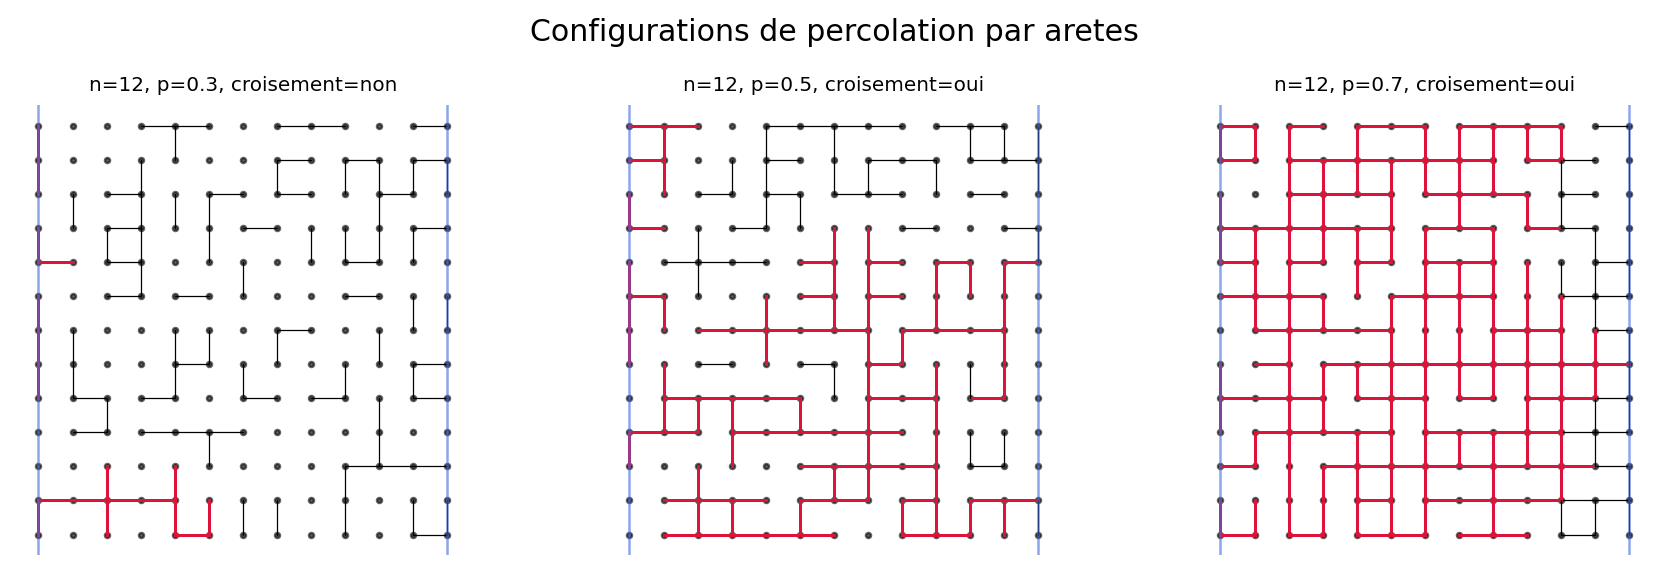
\includegraphics[width=0.95\textwidth]{figures/percolation_examples.png}
    \caption{Exemples de configurations de percolation par arêtes pour différentes valeurs de $p$.}
    \label{fig:percolation-examples}
\end{figure}

\section{Workflow de simulation}

La simulation peut être décomposée en cinq étapes principales.

\begin{figure}[H]
    \centering
    % Remplacer le nom du fichier ci-dessous par le nom exact de ton image si besoin.
    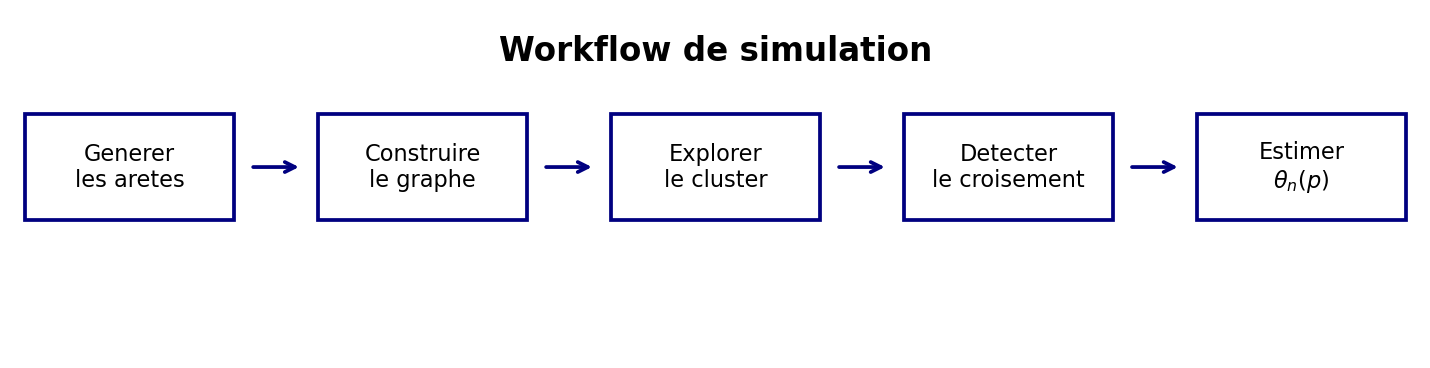
\includegraphics[width=0.85\textwidth]{figures/workflow.png}
    \caption{Workflow utilisé pour simuler le modèle de percolation et estimer la probabilité de croisement.}
    \label{fig:workflow}
\end{figure}

\begin{enumerate}
    \item Générer des variables de Bernoulli indépendantes pour toutes les arêtes.
    \item Construire le graphe induit par les arêtes ouvertes.
    \item Lancer une exploration à partir de tous les sommets du bord gauche.
    \item Utiliser un parcours en largeur pour identifier tous les sommets connectés au bord gauche.
    \item Vérifier si l'exploration atteint le bord droit.
\end{enumerate}

% ============================================================
% CHAPTER 2
% ============================================================
\chapter{Probabilité de croisement}

\section{Définition de \texorpdfstring{$\theta_n(p)$}{theta n p}}

\begin{definitionbox}{Probabilité de croisement}{theta}
Pour $n\in\N^*$ et $p\in[0,1]$, on définit
\[
\theta_n(p)=\Pbb(C_n),
\]
où $C_n$ désigne l'événement selon lequel le bord gauche est relié au bord droit par un chemin ouvert.
\end{definitionbox}

La fonction
\[
p\longmapsto \theta_n(p)
\]
mesure donc la probabilité d'observer un croisement dans une grille finie de taille $n$.

\section{Croissance de la probabilité de croisement}

\begin{theorembox}{Croissance de $\theta_n(p)$}{monotone}
Pour tout $n\in\N^*$ fixé, la fonction
\[
p\longmapsto \theta_n(p)
\]
est croissante sur $[0,1]$.
\end{theorembox}

\begin{proofbox}
Soit $(U_e)_{e\in E_n}$ une famille de variables aléatoires indépendantes suivant une loi uniforme sur $[0,1]$. Pour une probabilité $p$, on déclare l'arête $e$ ouverte si
\[
U_e\leq p.
\]
Si $p\leq p'$, alors toute arête ouverte au niveau $p$ est aussi ouverte au niveau $p'$, car
\[
U_e\leq p\leq p'.
\]
Ainsi, lorsque l'on passe de $p$ à $p'$, on peut ouvrir de nouvelles arêtes, mais on ne ferme aucune arête déjà ouverte. Donc tout croisement gauche-droite existant pour $p$ existe encore pour $p'$. On a donc
\[
C_n(p)\subset C_n(p').
\]
Par conséquent,
\[
\theta_n(p)=\Pbb(C_n(p))\leq \Pbb(C_n(p'))=\theta_n(p').
\]
La fonction $\theta_n$ est donc croissante.
\end{proofbox}

\section{Estimation Monte Carlo}

La probabilité $\theta_n(p)$ peut être estimée numériquement par répétition d'expériences indépendantes. Si $N_{\mathrm{sim}}$ configurations sont générées et si $Y_i$ désigne l'indicatrice d'un croisement pour la $i$-ième simulation, alors l'estimateur Monte Carlo est
\[
\widehat{\theta}_n(p)
=
\frac{1}{N_{\mathrm{sim}}}
\sum_{i=1}^{N_{\mathrm{sim}}}Y_i.
\]

\begin{propositionbox}{Estimateur sans biais}{unbiased}
L'estimateur Monte Carlo $\widehat{\theta}_n(p)$ est sans biais :
\[
\E[\widehat{\theta}_n(p)]=\theta_n(p).
\]
\end{propositionbox}

\begin{proofbox}
Comme $Y_i$ est l'indicatrice de l'événement $C_n$, on a
\[
\E[Y_i]=\Pbb(C_n)=\theta_n(p).
\]
Donc
\[
\E[\widehat{\theta}_n(p)]
=
\E\left[
\frac{1}{N_{\mathrm{sim}}}
\sum_{i=1}^{N_{\mathrm{sim}}}Y_i
\right]
=
\frac{1}{N_{\mathrm{sim}}}
\sum_{i=1}^{N_{\mathrm{sim}}}\E[Y_i]
=
\theta_n(p).
\]
\end{proofbox}

\begin{figure}[H]
    \centering
    % Remplacer le nom du fichier ci-dessous par le nom exact de ton image si besoin.
    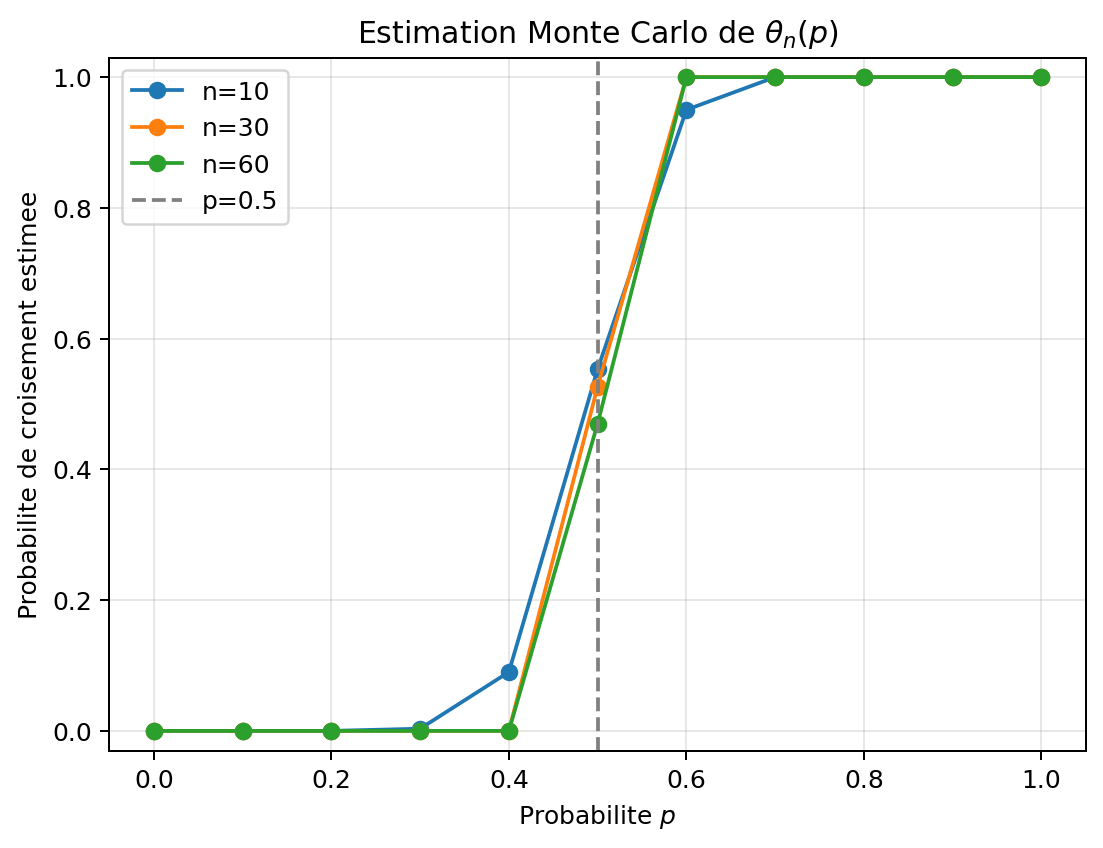
\includegraphics[width=0.8\textwidth]{figures/monte_carlo_theta.png}
    \caption{Estimation Monte Carlo de $\theta_n(p)$ pour différentes tailles de grille.}
    \label{fig:monte-carlo}
\end{figure}

\begin{propositionbox}{Variance et intervalle de confiance}{ci}
Comme $Y_i$ suit une loi de Bernoulli de paramètre $\theta_n(p)$, la variance de l'estimateur Monte Carlo est
\[
\Var(\widehat{\theta}_n(p))
=
\frac{\theta_n(p)(1-\theta_n(p))}{N_{\mathrm{sim}}}.
\]
Un intervalle de confiance approximatif à $95\%$ est donné par
\[
\widehat{\theta}_n(p)
\pm
1.96
\sqrt{
\frac{\widehat{\theta}_n(p)(1-\widehat{\theta}_n(p))}{N_{\mathrm{sim}}}
}.
\]
\end{propositionbox}

\section{Table de résultats numériques}

Le tableau suivant donne un exemple de résultats obtenus par simulation Monte Carlo avec $N_{\mathrm{sim}}=1000$ répétitions pour chaque couple $(n,p)$. Les valeurs peuvent légèrement varier selon la graine aléatoire utilisée. Les valeurs du tableau ne doivent pas nécessairement coïncider exactement avec celles de la figure, car elles dépendent du nombre de simulations, de la grille de valeurs de $p$ et de la graine aléatoire utilisée.

\begin{table}[H]
\centering
\begin{tabular}{c|ccc}
\toprule
\textbf{Taille $n$} & \textbf{$p=0.4$} & \textbf{$p=0.5$} & \textbf{$p=0.6$} \\
\midrule
$10$ & $0.104$ & $0.542$ & $0.935$ \\
$30$ & $0.003$ & $0.538$ & $0.999$ \\
$60$ & $0.000$ & $0.518$ & $1.000$ \\
\bottomrule
\end{tabular}
\caption{Estimations de $\theta_n(p)$ par simulation Monte Carlo avec $N_{\mathrm{sim}}=1000$.}
\label{tab:numerical-results}
\end{table}

\section{Interprétation des résultats numériques}

Les résultats numériques mettent en évidence un phénomène de transition. Pour $p=0.4$, la probabilité de croisement devient très faible lorsque la taille $n$ augmente. Cela signifie que les chemins ouverts restent généralement locaux et ne parviennent pas à relier les deux bords opposés.

Pour $p=0.6$, la probabilité de croisement devient presque égale à $1$ dès que la grille est suffisamment grande. Dans ce régime, les arêtes ouvertes sont assez nombreuses pour former un grand cluster traversant la grille.

La zone la plus intéressante se situe autour de $p=0.5$. Pour cette valeur, les simulations donnent une probabilité proche de $0.5$, ce qui traduit un équilibre entre l'existence d'un chemin ouvert gauche-droite et l'existence d'un chemin dual haut-bas. Lorsque $n$ augmente, la transition entre le régime sans croisement et le régime avec croisement devient de plus en plus abrupte.

\begin{remarkbox}{Interprétation statistique}{statinterp}
Le nombre de simulations contrôle la précision statistique, tandis que la taille $n$ contrôle l'échelle géométrique du problème. Augmenter $N_{\mathrm{sim}}$ réduit le bruit Monte Carlo. Augmenter $n$ rend la transition autour de la probabilité critique plus nette.
\end{remarkbox}

% ============================================================
% CHAPTER 3
% ============================================================
\chapter{Bornes et comportement critique}

\section{Une borne par comptage des chemins}

Une manière naturelle de majorer la probabilité de croisement consiste à compter les chemins ouverts possibles. Si un croisement gauche-droite existe, alors il existe au moins un chemin ouvert partant du bord gauche et de longueur au moins $n$.

\begin{propositionbox}{Borne de l'union pour les croisements}{unionbound}
Soit $N_k$ un majorant du nombre de chemins de longueur $k$ partant du bord gauche. Sur le réseau carré, on peut utiliser le majorant grossier
\[
N_k\leq (n+1)4^k.
\]
Cette borne est volontairement grossière : elle autorise des chemins avec retours en arrière et compte donc davantage de chemins que nécessaire. Elle suffit cependant pour obtenir une majoration simple.

Alors
\[
\theta_n(p)
\leq
\sum_{k\geq n}(n+1)4^k p^k.
\]
\end{propositionbox}

\begin{proofbox}
Pour un chemin fixé de longueur $k$, la probabilité que toutes ses arêtes soient ouvertes vaut $p^k$, par indépendance. Un croisement implique l'existence d'au moins un chemin ouvert de longueur au moins $n$ partant du bord gauche. Par la borne de l'union,
\[
\theta_n(p)
\leq
\sum_{k\geq n}N_kp^k.
\]
En utilisant $N_k\leq (n+1)4^k$, on obtient
\[
\theta_n(p)
\leq
\sum_{k\geq n}(n+1)(4p)^k.
\]
\end{proofbox}

\begin{theorembox}{Disparition de la probabilité de croisement pour $p$ petit}{smallp}
Si $p<1/4$, alors
\[
\lim_{n\to\infty}\theta_n(p)=0.
\]
\end{theorembox}

\begin{proofbox}
Si $p<1/4$, alors $4p<1$. D'après la borne précédente,
\[
\theta_n(p)
\leq
(n+1)\sum_{k\geq n}(4p)^k
=
(n+1)\frac{(4p)^n}{1-4p}.
\]
Comme $(4p)^n$ décroît exponentiellement vite, ce terme domine le facteur polynomial $n+1$. Ainsi,
\[
(n+1)(4p)^n\longrightarrow 0.
\]
Donc
\[
\theta_n(p)\longrightarrow 0.
\]
\end{proofbox}

\section{Probabilité critique}

\begin{definitionbox}{Probabilité critique}{pc}
La probabilité critique $p_c$ est la valeur qui sépare le régime sous-critique, où les longues connexions ouvertes sont peu probables, du régime surcritique, où les longues connexions deviennent probables.
\end{definitionbox}

Pour la percolation par arêtes sur le réseau carré infini, il est connu que
\[
p_c=\frac12.
\]
Dans le cadre fini, cette valeur apparaît numériquement comme le point autour duquel la probabilité de croisement passe rapidement de valeurs proches de $0$ à des valeurs proches de $1$.

\begin{remarkbox}{Effet de taille finie}{finite}
Pour une taille $n$ finie, la transition n'est pas parfaitement brutale. La courbe $p\mapsto\theta_n(p)$ est croissante et relativement lisse. Cependant, lorsque $n$ augmente, la zone de transition devient plus étroite, ce qui donne visuellement l'impression d'un seuil de plus en plus net.
\end{remarkbox}

\section{Interprétation du seuil critique}

Les simulations suggèrent que la valeur critique est proche de $1/2$. Ce n'est pas un hasard : pour la percolation par arêtes sur le réseau carré, le seuil critique exact est
\[
p_c=\frac12.
\]
L'idée intuitive repose sur l'auto-dualité du réseau carré. Lorsque $p=1/2$, les arêtes ouvertes et les arêtes fermées jouent des rôles symétriques.

\begin{theorembox}{Seuil critique du réseau carré}{critical}
Pour la percolation de Bernoulli par arêtes sur le réseau carré infini $\Z^2$, la probabilité critique est
\[
p_c=\frac12.
\]
\end{theorembox}

\begin{proofbox}
Une preuve complète de ce théorème dépasse le cadre de ce rapport, car elle nécessite des résultats plus profonds de la théorie de la percolation en dimension deux.

Dans ce rapport, l'argument de dualité sur un rectangle fini est utilisé pour motiver la valeur $p_c=1/2$. La preuve rigoureuse sur le réseau infini demande des outils supplémentaires de théorie de la percolation. Néanmoins, l'idée centrale est que, pour $p=1/2$, le modèle primal et le modèle dual ont la même loi. Les croisements ouverts gauche-droite et les croisements duaux haut-bas sont alors en équilibre.
\end{proofbox}

% ============================================================
% CHAPTER 4
% ============================================================
\chapter{Dualité planaire}

\section{Intuition du graphe dual}

Dans la percolation planaire, le graphe dual est obtenu en plaçant un sommet dual dans chaque face du graphe initial, puis en dessinant des arêtes duales qui traversent les arêtes du graphe primal. Une arête duale est ouverte exactement lorsque l'arête primale correspondante est fermée.

Cela crée une relation complémentaire entre les chemins ouverts dans le graphe primal et les chemins ouverts dans le graphe dual. Dans un rectangle fini, s'il n'existe pas de croisement ouvert gauche-droite dans le graphe primal, alors il existe un croisement dual haut-bas.

\begin{definitionbox}{Configuration duale}{dualconfig}
À partir d'une configuration de percolation de paramètre $p$, la configuration duale est obtenue en déclarant une arête duale ouverte lorsque l'arête primale correspondante est fermée. Ainsi, les arêtes duales sont ouvertes avec probabilité $1-p$.
\end{definitionbox}

\section{Figure de dualité}

La figure suivante illustre le principe de dualité. Les arêtes pleines représentent le graphe primal, tandis que les arêtes pointillées représentent le graphe dual. Un chemin primal gauche-droite empêche l'existence simultanée d'un chemin dual haut-bas, car les deux chemins devraient nécessairement se couper.

\begin{figure}[H]
\centering
\begin{tikzpicture}[scale=1.05]
    % primal grid
    \foreach \x in {0,1,2,3,4} {
        \foreach \y in {0,1,2,3} {
            \fill[black] (\x,\y) circle (1.5pt);
        }
    }

    % all primal edges light
    \foreach \x in {0,1,2,3} {
        \foreach \y in {0,1,2,3} {
            \draw[black!35] (\x,\y) -- (\x+1,\y);
        }
    }
    \foreach \x in {0,1,2,3,4} {
        \foreach \y in {0,1,2} {
            \draw[black!35] (\x,\y) -- (\x,\y+1);
        }
    }

    % primal open crossing highlighted
    \draw[line width=2.2pt, red!75!black] (0,1) -- (1,1);
    \draw[line width=2.2pt, red!75!black] (1,1) -- (1,2);
    \draw[line width=2.2pt, red!75!black] (1,2) -- (2,2);
    \draw[line width=2.2pt, red!75!black] (2,2) -- (3,2);
    \draw[line width=2.2pt, red!75!black] (3,2) -- (3,1);
    \draw[line width=2.2pt, red!75!black] (3,1) -- (4,1);

    % dual vertices
    \foreach \x in {0.5,1.5,2.5,3.5} {
        \foreach \y in {0.5,1.5,2.5} {
            \fill[blue!70!black] (\x,\y) circle (1.2pt);
        }
    }

    % dual edges dashed
    \foreach \x in {0.5,1.5,2.5} {
        \foreach \y in {0.5,1.5,2.5} {
            \draw[blue!60,dashed] (\x,\y) -- (\x+1,\y);
        }
    }
    \foreach \x in {0.5,1.5,2.5,3.5} {
        \foreach \y in {0.5,1.5} {
            \draw[blue!60,dashed] (\x,\y) -- (\x,\y+1);
        }
    }

    % labels
    \node[red!75!black, below] at (2,-0.55) {chemin primal ouvert gauche-droite};
    \node[blue!70!black, above] at (2,3.45) {arêtes duales pointillées};
    \draw[->, thick, red!75!black] (-0.7,1) -- (-0.1,1);
    \node[left, red!75!black] at (-0.7,1) {gauche};
    \draw[->, thick, red!75!black] (4.7,1) -- (4.1,1);
    \node[right, red!75!black] at (4.7,1) {droite};
\end{tikzpicture}
\caption{Illustration du graphe primal et du graphe dual dans une grille planaire. Les arêtes rouges représentent un chemin primal ouvert. Les arêtes bleues pointillées représentent le graphe dual. Un croisement primal gauche-droite bloque nécessairement un croisement dual haut-bas.}
\label{fig:duality-tikz}
\end{figure}

\section{Complémentarité des croisements}

\begin{theorembox}{Identité de dualité dans un rectangle fini}{duality}
Pour une grille rectangulaire adaptée et son dual, l'événement de croisement primal gauche-droite est complémentaire de l'événement de croisement dual haut-bas. Par conséquent,
\[
\theta_n(p)+\theta_n(1-p)=1.
\]
\end{theorembox}

\begin{proofbox}
La preuve repose sur la planarité. Un chemin primal ouvert traversant le rectangle de gauche à droite empêche tout chemin dual ouvert de traverser le rectangle de haut en bas, car les deux chemins devraient se croiser. À un point d'intersection, une arête primale et son arête duale correspondante ne peuvent pas être ouvertes simultanément, puisque l'arête duale est ouverte exactement lorsque l'arête primale est fermée.

Réciproquement, s'il n'existe pas de chemin primal ouvert de gauche à droite, on peut suivre la frontière séparant le cluster connecté au bord gauche du reste du rectangle. Cette frontière forme un chemin ouvert dans le graphe dual reliant le haut au bas.

Ainsi, exactement l'un des deux événements suivants se produit :
\begin{itemize}
    \item un croisement ouvert gauche-droite dans le graphe primal ;
    \item un croisement ouvert haut-bas dans le graphe dual.
\end{itemize}
Comme le graphe dual a pour paramètre $1-p$, la probabilité du second événement est $\theta_n(1-p)$. On obtient donc
\[
\theta_n(p)+\theta_n(1-p)=1.
\]
\end{proofbox}

\begin{remarkbox}{Pourquoi $p=1/2$ est particulier}{half}
Si $p=1/2$, alors $1-p=p$. L'identité de dualité donne
\[
\theta_n(1/2)+\theta_n(1/2)=1,
\]
donc
\[
\theta_n(1/2)=\frac12.
\]
Cela explique pourquoi la probabilité de croisement observée empiriquement est proche de $0.5$ autour de $p=0.5$.
\end{remarkbox}

% ============================================================
% CHAPTER 5
% ============================================================
\chapter{Implémentation algorithmique}

\section{Parcours en largeur}

L'objectif informatique est de déterminer s'il existe un chemin ouvert reliant le bord gauche au bord droit. Il s'agit d'un problème d'exploration de graphe.

\begin{definitionbox}{Parcours en largeur}{bfs}
Le parcours en largeur, ou \textit{Breadth-First Search} (BFS), est un algorithme qui explore un graphe couche par couche. À partir d'un ensemble de sommets initiaux, il visite d'abord leurs voisins, puis les voisins de ces voisins, et ainsi de suite.
\end{definitionbox}

Dans le problème de percolation, le BFS démarre depuis tous les sommets du bord gauche et ne se déplace qu'à travers les arêtes ouvertes. Si l'exploration atteint le bord droit, alors il existe un croisement gauche-droite.

\subsection*{Workflow algorithmique}

\begin{enumerate}
    \item Générer indépendamment toutes les arêtes horizontales et verticales avec probabilité $p$.
    \item Initialiser une file avec tous les sommets du bord gauche.
    \item Explorer les sommets voisins uniquement à travers les arêtes ouvertes.
    \item Marquer chaque sommet visité afin d'éviter les boucles et les répétitions.
    \item Si un sommet du bord droit est atteint, retourner \texttt{True}.
    \item Si la file devient vide, retourner \texttt{False}.
\end{enumerate}

\section{Complexité}

Soient $|V_n|$ le nombre de sommets et $|E_n|$ le nombre d'arêtes. Le parcours en largeur explore chaque sommet et chaque arête ouverte au plus une fois. Sa complexité est donc
\[
O(|V_n|+|E_n|).
\]
Pour une grille $n\times n$,
\[
|V_n|=(n+1)^2,
\qquad
|E_n|=2n(n+1).
\]
La complexité est donc d'ordre
\[
O(n^2).
\]

\section{Choix d'implémentation}

L'implémentation évite les difficultés liées au \textit{splicing} en séparant les arêtes horizontales et verticales :
\begin{itemize}
    \item les arêtes horizontales sont stockées dans une matrice de taille $(n+1)\times n$ ;
    \item les arêtes verticales sont stockées dans une matrice de taille $n\times(n+1)$.
\end{itemize}

\begin{remarkbox}{Amélioration pratique}{implementation}
Au lieu de forcer toutes les arêtes dans une seule matrice artificielle, séparer les arêtes horizontales et verticales rend le code plus clair, réduit les erreurs d'indexation et améliore la lisibilité de la simulation.
\end{remarkbox}

% ============================================================
% CHAPTER 6
% ============================================================
\chapter{Validation, limites et extensions}

\section{Validation de la simulation}

Plusieurs vérifications permettent de s'assurer que l'implémentation est cohérente :
\begin{itemize}
    \item lorsque $p=0$, aucune arête n'est ouverte, donc la probabilité de croisement doit être nulle ;
    \item lorsque $p=1$, toutes les arêtes sont ouvertes, donc la probabilité de croisement doit être égale à $1$ ;
    \item lorsque $p$ augmente, la probabilité de croisement estimée doit globalement augmenter, à de petites fluctuations Monte Carlo près ;
    \item autour de $p=1/2$, la probabilité de croisement doit être proche de $1/2$ pour des rectangles symétriques.
\end{itemize}

\begin{remarkbox}{Fiabilité numérique}{reliability}
Les méthodes Monte Carlo sont aléatoires : deux exécutions peuvent donner des valeurs légèrement différentes. Pour rendre les résultats reproductibles, l'implémentation utilise une graine aléatoire. Pour améliorer la précision, on peut augmenter le nombre de simulations.
\end{remarkbox}

\section{Limites du projet}

Le modèle étudié est volontairement simple. Il se concentre sur une percolation par arêtes indépendante sur une grille régulière finie. Ce cadre est riche mathématiquement, mais présente plusieurs limites :
\begin{itemize}
    \item seules des grilles finies sont simulées, alors que la transition de phase théorique est un phénomène de volume infini ;
    \item les arêtes sont supposées indépendantes, ce qui n'est pas toujours réaliste dans des applications de réseaux réels ;
    \item la simulation se concentre sur les croisements gauche-droite et n'analyse pas entièrement la distribution des tailles de clusters ;
    \item la convergence vers le comportement du réseau infini est seulement observée numériquement.
\end{itemize}

\section{Extensions possibles}

Plusieurs prolongements pourraient enrichir le projet :
\begin{itemize}
    \item étudier la percolation par sites, où ce sont les sommets et non les arêtes qui sont ouverts ou fermés ;
    \item estimer la distribution de la taille du plus grand cluster ;
    \item calculer la taille moyenne des clusters en fonction de $p$ ;
    \item comparer le parcours en largeur avec un algorithme Union-Find ;
    \item réaliser des simulations Monte Carlo plus larges pour observer le \textit{finite-size scaling} ;
    \item étendre la simulation à d'autres graphes, comme les réseaux triangulaires, hexagonaux ou aléatoires.
\end{itemize}

\section{Intérêt professionnel}

Les modèles de percolation dépassent le cadre de la théorie des probabilités. Ils apparaissent en science des réseaux, en épidémiologie, en science des matériaux, en analyse de fiabilité et en physique statistique. Ils permettent d'étudier comment des connexions locales aléatoires peuvent produire une connectivité globale, une fragmentation ou une transition de phase.

Ce projet illustre donc un workflow complet : définir un modèle mathématique, implémenter une simulation, estimer une probabilité numériquement, valider les résultats et les interpréter à l'aide d'outils théoriques.

\section{Alternative algorithmique : Union-Find}

Une autre approche possible consiste à utiliser une structure de données Union-Find. À chaque arête ouverte, on fusionne les deux composantes contenant ses extrémités. Il suffit ensuite de vérifier si une composante connecte un sommet du bord gauche à un sommet du bord droit. Cette méthode est particulièrement efficace lorsque l'on souhaite répéter de nombreuses simulations, suivre l'évolution des composantes connexes ou analyser la taille des clusters.

Dans le cadre de ce rapport, le parcours en largeur a été privilégié car il est simple à interpréter et directement relié à la recherche d'un chemin ouvert. L'algorithme Union-Find constitue néanmoins une extension naturelle pour rendre la simulation plus efficace à grande échelle.

\section{Compétences développées}

Ce projet a permis de mobiliser plusieurs compétences importantes :
\begin{itemize}
    \item modélisation probabiliste à partir de variables de Bernoulli ;
    \item simulation Monte Carlo et estimation numérique d'une probabilité ;
    \item exploration de graphes avec un parcours en largeur ;
    \item interprétation d'un phénomène de transition de phase ;
    \item implémentation Python structurée et reproductible ;
    \item validation numérique et analyse critique des limites du modèle.
\end{itemize}

% ============================================================
% CONCLUSION
% ============================================================
\chapter*{Conclusion}
\addcontentsline{toc}{chapter}{Conclusion}

Ce projet a étudié la percolation par arêtes à travers une approche à la fois théorique et computationnelle. Le modèle a été défini à l'aide de variables aléatoires de Bernoulli indépendantes attachées aux arêtes d'une grille finie. L'événement principal étudié était l'existence d'un chemin ouvert gauche-droite, dont la probabilité est notée $\theta_n(p)$.

La partie théorique a permis d'établir plusieurs propriétés importantes. Premièrement, $\theta_n(p)$ est croissante par rapport à $p$. Deuxièmement, un argument de comptage des chemins fournit une borne montrant que les croisements deviennent improbables pour des valeurs suffisamment petites de $p$. Enfin, la dualité planaire donne l'identité centrale
\[
\theta_n(p)+\theta_n(1-p)=1,
\]
qui explique le rôle particulier de $p=1/2$.

Les simulations numériques confirment le phénomène de transition attendu. Pour des petites probabilités, les croisements sont rares ; pour des grandes probabilités, ils deviennent presque certains ; et autour de $p=1/2$, la probabilité de croisement est proche de $1/2$. Lorsque la taille de la grille augmente, la transition devient plus nette.

Ainsi, ce projet montre comment la théorie des probabilités, les algorithmes de graphes et la simulation numérique peuvent être combinés pour analyser un modèle mathématique ayant une structure géométrique riche.

% ============================================================
% APPENDIX
% ============================================================
\appendix

\chapter{Code Python}

Le code Python suivant implémente la simulation de la percolation par arêtes, détecte les croisements gauche-droite par parcours en largeur et estime la probabilité de croisement par simulation Monte Carlo.

\begin{lstlisting}[caption={Simulation de la percolation par aretes en Python},label={lst:percolation-python}]
import numpy as np
from collections import deque


def generate_bond_percolation(n, p, rng=None):
    """
    Genere une configuration de percolation par aretes sur une grille n x n.

    Les sommets sont indexes par (i, j), avec i, j dans {0, ..., n}.

    horizontal[i, j] represente l'arete entre (i, j) et (i, j+1).
    vertical[i, j] represente l'arete entre (i, j) et (i+1, j).
    """
    if rng is None:
        rng = np.random.default_rng()

    horizontal = rng.random((n + 1, n)) < p
    vertical = rng.random((n, n + 1)) < p

    return horizontal, vertical


def has_left_right_crossing(horizontal, vertical):
    """
    Verifie s'il existe un chemin ouvert du bord gauche
    vers le bord droit en utilisant un parcours en largeur.
    """
    n = horizontal.shape[1]
    visited = np.zeros((n + 1, n + 1), dtype=bool)
    queue = deque()

    # Initialisation avec tous les sommets du bord gauche
    for i in range(n + 1):
        visited[i, 0] = True
        queue.append((i, 0))

    while queue:
        i, j = queue.popleft()

        # Si le bord droit est atteint, un croisement existe
        if j == n:
            return True

        # Deplacement vers la gauche
        if j > 0 and horizontal[i, j - 1] and not visited[i, j - 1]:
            visited[i, j - 1] = True
            queue.append((i, j - 1))

        # Deplacement vers la droite
        if j < n and horizontal[i, j] and not visited[i, j + 1]:
            visited[i, j + 1] = True
            queue.append((i, j + 1))

        # Deplacement vers le haut
        if i > 0 and vertical[i - 1, j] and not visited[i - 1, j]:
            visited[i - 1, j] = True
            queue.append((i - 1, j))

        # Deplacement vers le bas
        if i < n and vertical[i, j] and not visited[i + 1, j]:
            visited[i + 1, j] = True
            queue.append((i + 1, j))

    return False


def estimate_theta(n, p, simulations=1000, seed=42):
    """
    Estime theta_n(p), la probabilite d'un croisement gauche-droite,
    par simulation Monte Carlo.
    """
    rng = np.random.default_rng(seed)
    crossings = 0

    for _ in range(simulations):
        horizontal, vertical = generate_bond_percolation(n, p, rng)
        if has_left_right_crossing(horizontal, vertical):
            crossings += 1

    return crossings / simulations


def confidence_interval(theta_hat, simulations, level=1.96):
    """
    Renvoie un intervalle de confiance approximatif a 95% pour theta_hat.
    """
    standard_error = np.sqrt(theta_hat * (1 - theta_hat) / simulations)
    lower = max(0.0, theta_hat - level * standard_error)
    upper = min(1.0, theta_hat + level * standard_error)
    return lower, upper


if __name__ == "__main__":
    sizes = [10, 30, 60]
    probabilities = [0.4, 0.5, 0.6]
    simulations = 1000

    for n in sizes:
        print(f"n = {n}")
        for p in probabilities:
            theta_hat = estimate_theta(n, p, simulations=simulations)
            ci_low, ci_high = confidence_interval(theta_hat, simulations)
            print(
                f"p = {p:.2f}, theta_hat = {theta_hat:.3f}, "
                f"95% CI = [{ci_low:.3f}, {ci_high:.3f}]"
            )
        print("-" * 60)
\end{lstlisting}

% ============================================================
% BIBLIOGRAPHY
% ============================================================
\chapter*{Bibliographie}
\addcontentsline{toc}{chapter}{Bibliographie}

\begin{enumerate}
    \item G. Grimmett, \textit{Percolation}, Springer, 1999.
    \item H. Kesten, \textit{Percolation Theory for Mathematicians}, Birkhäuser, 1982.
    \item B. Bollobás and O. Riordan, \textit{Percolation}, Cambridge University Press, 2006.
\end{enumerate}

\end{document}
